\documentclass{beamer}

\usepackage[lined,ruled]{algorithm2e}
\usepackage{subfigure}
\usepackage[english]{babel}
\usepackage[latin1]{inputenc}
\usepackage{times}
\usepackage[T1]{fontenc} 
\usepackage{color}
\usepackage[absolute,overlay]{textpos}

\usetheme[secheader]{Boadilla}
\usefonttheme[onlylarge]{structurebold}
\setbeamerfont*{frametitle}{size=\normalsize,series=\bfseries}
\setbeamertemplate{navigation symbols}{}
\setbeamertemplate{mini frames}[box]
\setbeamertemplate{sections/subsections in toc}[square]
\setbeamertemplate{blocks}[rounded][shadow=true]
\setbeamertemplate{bibliography item}[text]

\setbeamercolor{lightorange}{fg=black,bg=orange!40}
\setbeamercolor{lightblue}{fg=black,bg=blue!30}

\newenvironment{colorblock}[2]
{\setbeamercolor{item}{fg=#1,bg=#1}\begin{beamerboxesrounded}[upper=#1,lower=#2,shadow=true]}
  {\end{beamerboxesrounded}}



% Setup TikZ

\usepackage{tikz}
\usetikzlibrary{arrows}
\tikzstyle{block}=[draw opacity=0.7,line width=1.4cm]


%%%%%%%%%%%%%%%%%%%%%%%%%%%%%%%%%%%%%
%%%%%%%%%%%%%%%%%%%%%%%%%%%%%%%%%%%%%
%%%%%%%%%%%%%%%%%%%%%%%%%%%%%%%%%%%%%

\newtheorem{observation}[theorem]{Observation} 

%%%%%%%%%%%%%%%%%%%%%%%%%%%%%%%%%%%%%
%%%%%%%%%%%%%%%%%%%%%%%%%%%%%%%%%%%%%
%%%%%%%%%%%%%%%%%%%%%%%%%%%%%%%%%%%%%

\title{Coordinating Distributed Systems}
\subtitle{Theory and practice}
\author{Daniele Venzano}
\institute{Eurecom}
\date


\begin{document}

\begin{frame}
  \titlepage
\end{frame}

%%%%%%%%%%%%%%%%%%%%%%%%%%%%%%%%%%%%%%%%%%%%%%%%%%%%%%%%%%
%%%%%%%%%%%%%%%%%%%%%%%%%%%%%%%%%%%%%%%%%%%%%%%%%%%%%%%%%%
\section{Introduction}

\begin{frame}
 \begin{colorblock}{blue}{lightblue}{ }
  \begin{center}
    \Huge \textbf{\texttt{Introduction}}
  \end{center}
  \end{colorblock}
\end{frame}

%%%%%%%%%%%%%%%%%%%%%%%%%%%%%%%%%%%%%%%%%%%%%%%%%%%%%%%%%%
\frame {\frametitle{Outline}
	\begin{itemize}
		\item \textbf{What is a distributed system?}
		
		\vspace{7pt}
		
		\item \textbf{The consensus problem}
		\begin{itemize}
			\item A few examples of distributed consensus
			\item CAP theorem
			\item Eventually consistent Vs Strongly consistent
			\item Fault tolerance: possible faults in distributed systems
		\end{itemize}
		
		\vspace{7pt}
		
		\item \textbf{Consensus protocols}
		\begin{itemize}
			\item Two phase commit
			\item Paxos overview
			\item Raft from A to Z
		\end{itemize}
		
		\vspace{7pt}
		
		\item \textbf{Implementations - ZooKeeper}
		\begin{itemize}
			\item History
			\item Architecture
			\item Data model
			\item Higher-level primitives
		\end{itemize}
			
	\end{itemize}
}
%%%%%%%%%%%%%%%%%%%%%%%%%%%%%%%%%%%%%%%%%%%%%%%%%%%%%%%%%%
\subsection{What is a distributed system?}
\frame {\frametitle{What is a distributed system?}
	\begin{center}
		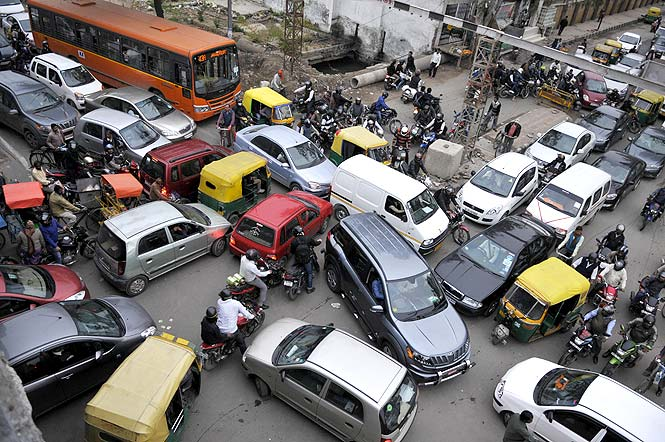
\includegraphics[width=0.6\textwidth]{images/traffic-jam}
	\end{center}
	\begin{itemize}
		\item A set of processes seeking to achieve some common goal by communicating with each other
	\end{itemize}
}

%%%%%%%%%%%%%%%%%%%%%%%%%%%%%%%%%%%%%%%%%%%%%%%%%%%%%%%%%%
\frame {\frametitle{What is a distributed system?}
	\begin{itemize}
		\item Like a software matrioshka
		\begin{itemize}
			\item Multi-threaded process
			\item Multi-process on a single server
			\item \textbf{Multiple processes in a set of servers in the same datacenter}
			\item \textbf{Multiple processes in a set of geographically distributed servers}
		\end{itemize}
	
		\vspace{10pt}
	
		\item Why?
		\begin{itemize}
			\item Inherent distribution (sensors, peer-to-peer, publish-subscribe, ...)
			\item Engineering choice (fault tolerance, replication, performance, ...)
		\end{itemize}
	
		\vspace{10pt}
		
		\item These processes need to coordinate to reach a common goal:
		\begin{itemize}
			\item data aggregation
			\item synchronization
			\item transactions
			\item ...
		\end{itemize}
	\end{itemize}
}

%%%%%%%%%%%%%%%%%%%%%%%%%%%%%%%%%%%%%%%%%%%%%%%%%%%%%%%%%%
%%%%%%%%%%%%%%%%%%%%%%%%%%%%%%%%%%%%%%%%%%%%%%%%%%%%%%%%%%

\section{The consensus problem}
\begin{frame}
 \begin{colorblock}{blue}{lightblue}{ }
  \begin{center}
    \Huge \textbf{\texttt{The consensus problem}}
  \end{center}
  \end{colorblock}
\end{frame}

%%%%%%%%%%%%%%%%%%%%%%%%%%%%%%%%%%%%%%%%%%%%%%%%%%%%%%%%%%
\subsection{Examples of the consensus problem}
\frame {\frametitle{Wedding consensus}
	\begin{itemize}
		\item The priest follows a well known protocol to reach a consensus:
		\begin{enumerate}
			\item Priest: Alice, will you marry Bob ?
			\item Alice: yes
			\item Priest: Bob, will you marry Alice ?
			\item Bob: yes
			\item Priest: You are now husband and wife
		\end{enumerate}

		\vspace{10pt}

		\item In distributed systems this becomes:
		\begin{enumerate}
			\item Coordinator: Alice, can you commit key X with value 5 ?
			\item Alice: yes, I can
			\item Coordinator: Bob, can you commit key X with value 5 ?
			\item Bob: yes, I can
			\item Coordinator: Ok, both of you record that X has now a value of 5
		\end{enumerate}

		\vspace{10pt}

		\item What if Bob flees from the church?
	\end{itemize}
}
%%%%%%%%%%%%%%%%%%%%%%%%%%%%%%%%%%%%%%%%%%%%%%%%%%%%%%%%%%
\frame {\frametitle{The two generals}
	\begin{center}
		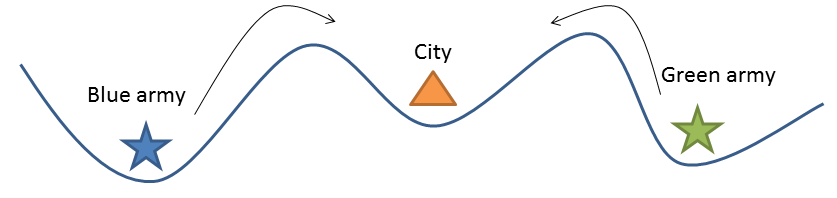
\includegraphics[width=\textwidth]{images/2generals}
	\end{center}
	\begin{itemize}
	\item Two generals want to attack a city
	\item They can only use unreliable messengers to communicate
	\item They need to attack at the same time to succeed
	\end{itemize}

	An infinite number of messages is needed for each general to be sure the other agrees on the time of the attack.
}

%%%%%%%%%%%%%%%%%%%%%%%%%%%%%%%%%%%%%%%%%%%%%%%%%%%%%%%%%%
\frame {\frametitle{Consensus examples}
	Processes need to reach a common goal:
	\begin{itemize}
		\item aggregate functions: sensors calculating average temperature
		\item synchronization: agree on a value, elect a leader
		\item reliable broadcast: a message sent to a group is received by all or none
		\item atomic commit: ensure that processes reach a common decision whether to commit or abort a transaction
		\item leader election: ensure there is only one process in charge at a given time
	\end{itemize}
}

%%%%%%%%%%%%%%%%%%%%%%%%%%%%%%%%%%%%%%%%%%%%%%%%%%%%%%%%%%
\frame {\frametitle{Properties of a distributed system}
	\begin{itemize}
		\item Linearizability\footnote{The CAP theorem calls Consistency what is actually Linearizability}: a given set of operations is \emph{linearizable} if it appears to the rest of the system to occur instantaneously
		\begin{itemize}
			\item Writes are linearizable operations if every read receives the most recent write or an error
		\end{itemize}
		\item Availability: a system is \emph{available} if every request to a non-failing node always receives a response, eventually
		\begin{itemize}
			\item Reading stale data is ok, though
		\end{itemize}
		\item Partition tolerance
		\begin{itemize}
			\item The system continues to function properly even if the network loses or delays an arbitrary number of messages
		\end{itemize}
	\end{itemize}

	The CAP theorem links these three properties.
}

%%%%%%%%%%%%%%%%%%%%%%%%%%%%%%%%%%%%%%%%%%%%%%%%%%%%%%%%%%
\frame {\frametitle{CAP theorem - 1}
	The theorem says: between C A P, you can choose only two
	\begin{center}
		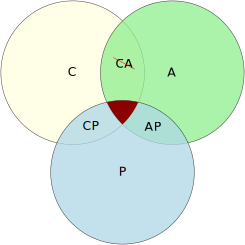
\includegraphics[width=0.5\textwidth]{images/cap}
	\end{center}
	(... but you need the P ...)
}

%%%%%%%%%%%%%%%%%%%%%%%%%%%%%%%%%%%%%%%%%%%%%%%%%%%%%%%%%%
\frame {\frametitle{CAP theorem - 2 - Why not all three?}
	\begin{center}
		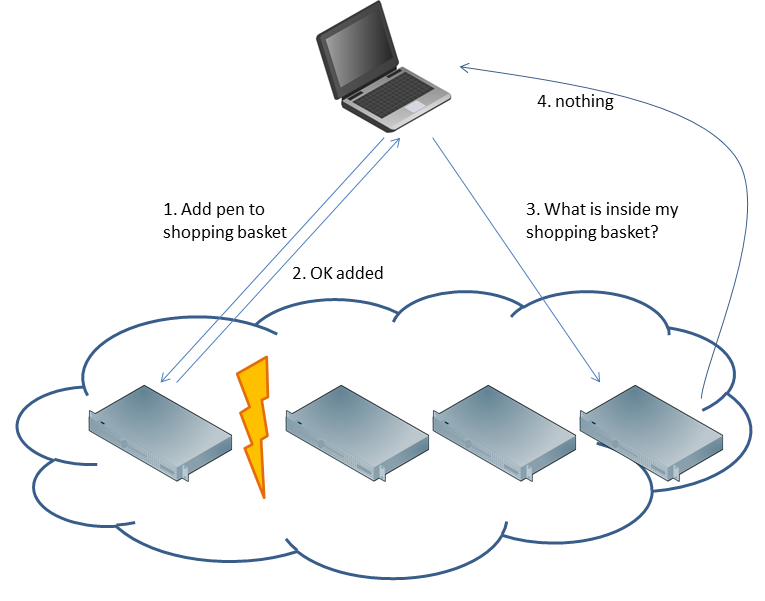
\includegraphics[width=0.6\textwidth]{images/cap2}
	\end{center}

	If there is a network partition either C or A will break
}

%%%%%%%%%%%%%%%%%%%%%%%%%%%%%%%%%%%%%%%%%%%%%%%%%%%%%%%%%%
\frame {\frametitle{CAP theorem - 3 - P}
	\begin{itemize}
		\item Network partitions occur outside anyone's control in real life
		\item Cannot sacrifice the Partition-Tolerance property
		\item In the event of a network partition either A or C is maintained: it is the choice of the designer
		\item Practical distributed systems are CP or AP
		\item Some can be configured to shift between CP and AP (tunable consistency)
	\end{itemize}
	
	\vspace{10pt}
	
	Note: a network partition can also be a very slow link
}

%%%%%%%%%%%%%%%%%%%%%%%%%%%%%%%%%%%%%%%%%%%%%%%%%%%%%%%%%%
\frame {\frametitle{CAP theorem - 4 - Summary}
	\begin{itemize}
		\item First stated by Eric Brewer (Berkeley) at the PODC 2000 keynote
		\item Formally proved by Gilbert and Lynch, 2002\cite{Gilbert02}
	\end{itemize}
	
	\vspace{5pt}

	\begin{itemize}
		\item The CAP theorem formally states the trade-offs among different distributed systems properties
		\item In practice network Partitions occur, the designer can choose one of Consistency or Availability
		\item The choice heavily depends on what your application/business logic is
	\end{itemize}
}

%%%%%%%%%%%%%%%%%%%%%%%%%%%%%%%%%%%%%%%%%%%%%%%%%%%%%%%%%%
\frame {\frametitle{CAP theorem - 5 - Summary}

	CP-oriented systems:
	\begin{itemize}
		\item BigTable, Hbase, MongoDB, Redis, MemCacheDB, Scalaris, Paxos, ZooKeeper$^1$
	\end{itemize}
	
	\vspace{5pt}
	
	AP-oriented systems:
	\begin{itemize}
		\item Amazon Dynamo, CouchDB, Cassandra\footnote{CA or CP tunable}, SimpleDB, Riak, Voldemort
	\end{itemize}

	In-depth articles on the misuse of the CAP theorem in describing real systems:
	\begin{itemize}
	\item \url{https://codahale.com/you-cant-sacrifice-partition-tolerance/}
	\item \url{https://martin.kleppmann.com/2015/05/11/please-stop-calling-databases-cp-or-ap.html}
	\end{itemize}
}

%%%%%%%%%%%%%%%%%%%%%%%%%%%%%%%%%%%%%%%%%%%%%%%%%%%%%%%%%%
\frame {\frametitle{Consistency models}

	\begin{itemize}
		\item Eventual consistency: after a write, every read from the distributed system will \emph{eventually} return the written value, if no new updates are made to it
	
		\vspace{5pt}
	
		\item Strong consistency: after a write, all reads from the distributed system will return either the old or the new value
	\end{itemize}
}

%%%%%%%%%%%%%%%%%%%%%%%%%%%%%%%%%%%%%%%%%%%%%%%%%%%%%%%%%%
\frame {\frametitle{Fault tolerance in distributed systems}
	Faults examples:
	\begin{itemize}
		\item Simple: network partitions, hardware or software crashes, outdated/malicious nodes (bizantine faults)
		\item Complex: feedback loops that overcompensate in good faith (examples in next slides)
	\end{itemize}

	Faults will always happen, design tolerance mechanisms:
	\begin{itemize}
		\item Replication: master-slave ($\rightarrow$ failover) or load balancing
		\item Isolation: malfunctioning components do not affect the system as a whole
	\end{itemize}
}

%%%%%%%%%%%%%%%%%%%%%%%%%%%%%%%%%%%%%%%%%%%%%%%%%%%%%%%%%%
\frame {\frametitle{Amazon DynamoDB crash (2015/09/20)}
	DynamoDB: distributed NoSQL database from Amazon web services (AWS)
	\begin{enumerate}
		\item Network disruption caused timeouts of some storage servers
		\item The affected servers tried to re-establish their membership
		\item A change of usage pattern caused membership data to be unexpectedly large
		\item Membership servers started to overload
		\item More storage servers timed-out on health checks to membership servers
		\item Cascading failure, stabilized at 55\% error rate for customers
	\end{enumerate}
	Post-mortem: \url{https://aws.amazon.com/message/5467D2/}
}

%%%%%%%%%%%%%%%%%%%%%%%%%%%%%%%%%%%%%%%%%%%%%%%%%%%%%%%%%%
\frame {\frametitle{More real-world failures}
	\begin{itemize}
		\item Google: \url{https://status.cloud.google.com/summary}
		\item Facebook: \url{https://www.facebook.com/notes/facebook-engineering/more-details-on-todays-outage/431441338919}
		\item Apple: \url{http://appleinsider.com/articles/16/06/02/apples-app-stores-apple-tv-itunes-other-services-hit-with-downtime}
		\item Microsoft (Azure): \url{https://azure.microsoft.com/en-us/status/history/}
	\end{itemize}
}

%%%%%%%%%%%%%%%%%%%%%%%%%%%%%%%%%%%%%%%%%%%%%%%%%%%%%%%%%%
%%%%%%%%%%%%%%%%%%%%%%%%%%%%%%%%%%%%%%%%%%%%%%%%%%%%%%%%%%

\section{Consensus protocols}

\begin{frame}
 \begin{colorblock}{blue}{lightblue}{ }
  \begin{center}
    \Huge \textbf{\texttt{Consensus protocols}}
  \end{center}
  \end{colorblock}
\end{frame}

%%%%%%%%%%%%%%%%%%%%%%%%%%%%%%%%%%%%%%%%%%%%%%%%%%%%%%%%%%
\subsection{Overview}
\frame {\frametitle{Consensus protocols overview}
	Simplest (but unsafe):
	\begin{itemize}
		\item Two-phase commit
	\end{itemize}

	\vspace{7pt}

	Traditionally studied for modern distributed systems:
	\begin{itemize}
		\item Paxos
		\item Raft
		\item ZAB
	\end{itemize}

	\vspace{7pt}
	
	Other:
	\begin{itemize}
		\item Lock-step (used in some multiplayer video games)
		\item The proof-of-work from Bitcoin
	\end{itemize}
}

%%%%%%%%%%%%%%%%%%%%%%%%%%%%%%%%%%%%%%%%%%%%%%%%%%%%%%%%%%
\subsection{Two-phase commit}
\frame {\frametitle{Two-phase commit}
	Simplest protocol for consensus
	\begin{center}
		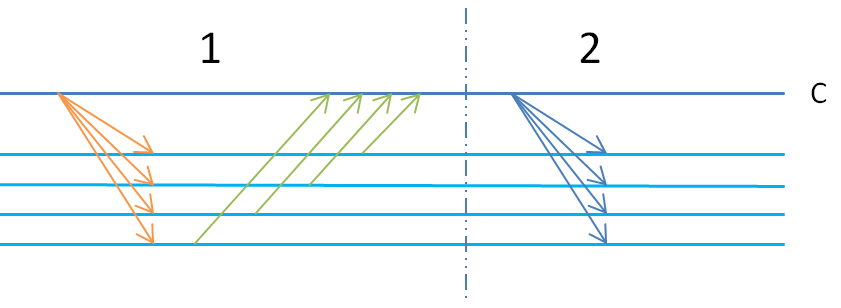
\includegraphics[width=0.8\textwidth]{images/2phasecommit}
	\end{center}

	\begin{itemize}
		\item Phase 1
		\begin{itemize}
			\item One coordinator node \emph{C} suggests a value to the other nodes
			\item C gathers the responses
		\end{itemize}
		\item Phase 2
		\begin{itemize}
			\item If all nodes agree, C sends a commit command, abort otherwise
		\end{itemize}
	\end{itemize}

}

%%%%%%%%%%%%%%%%%%%%%%%%%%%%%%%%%%%%%%%%%%%%%%%%%%%%%%%%%%
\frame {\frametitle{Two-phase commit - Why it is not enough?}
Two phase commit cannot make progress if there are simple failures.\cite{2PCarticle}
	
	\begin{center}
	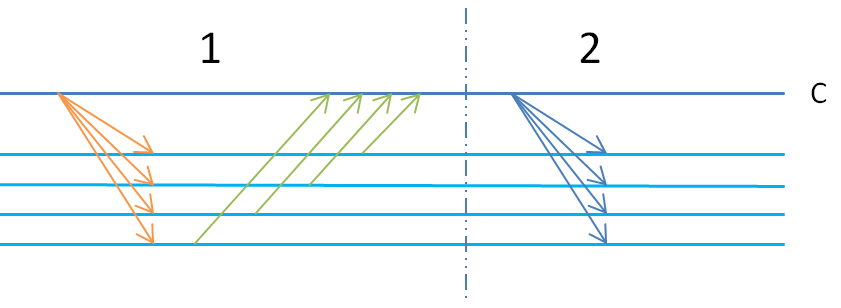
\includegraphics[width=0.6\textwidth]{images/2phasecommit}
	\end{center}
	
	\begin{itemize}
		\item If C fails, nothing can be done until it is restarted
		\begin{itemize}
			\item If C fails in phase 1, it has to abort the commit and retry
			\item If C fails in phase 2, it has to replay the outcome (commit/abort)
			\item In both cases the outcome is uncertain until C restarts
		\end{itemize}
		\item If just one of the other nodes crashes, is slow or unreachable, the value cannot be committed.
	\end{itemize}	
}

%%%%%%%%%%%%%%%%%%%%%%%%%%%%%%%%%%%%%%%%%%%%%%%%%%%%%%%%%%
\subsection{State-machine replication}
\frame {\frametitle{State-machine replication}
	\begin{center}
		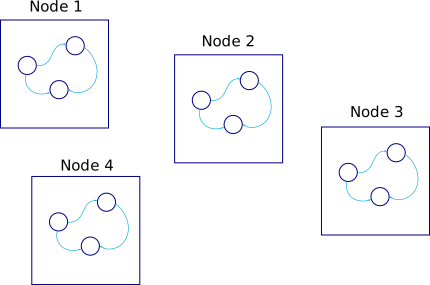
\includegraphics[width=0.4\textwidth]{images/dist-state-machine}
	\end{center}
	
	\begin{itemize}
		\item Paxos and Raft use distributed state machines
		\item State machines are fully deterministic
		\item Committed operations are executed by all state machines in the cluster in the same order
	\end{itemize}

	Example operation: set variable $x$ to value $5$
}

%%%%%%%%%%%%%%%%%%%%%%%%%%%%%%%%%%%%%%%%%%%%%%%%%%%%%%%%%%
\subsection{Paxos}
\frame {\frametitle{Paxos}
	Old and well-known family of protocols for distributed consensus.
	\begin{itemize}
		\item first presented in 1989, paper published in 1998\cite{LamportPaxos1}
		\item has been formally proven to be safe
	\end{itemize}

	\vspace{5pt}
	
	Complex and difficult to implement
	\begin{itemize}
		\item Basic Paxos protocol decides on a single output value
		\item Multi-Paxos extends the Basic protocol for practical use
		\item Many variants: cheap, fast, generalized, byzantine
		\item No reference implementation
		\item Many papers try to make it more approachable\cite{LampsonPaxos, PaxosMadeSimple, PaxosMadeLive}
		\item Paxos needs a large enough subnet to be non-faulty for a long enough time, otherwise it might never terminate
	\end{itemize}
	
}

%%%%%%%%%%%%%%%%%%%%%%%%%%%%%%%%%%%%%%%%%%%%%%%%%%%%%%%%%%
\frame {\frametitle{A Paxos round - 1}
	\begin{center}
		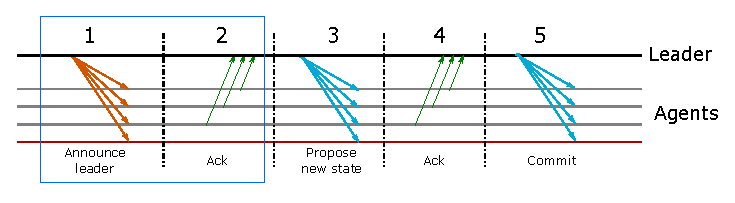
\includegraphics[width=0.8\textwidth]{images/paxos-round1}
	\end{center}

	Phase 1 of a very simplified Paxos round:
	\begin{itemize}
		\item A node in the cluster self-appoints leader and chooses a new ballot ID
		\item Sends a ballot proposal to the other nodes (1)
		\item The other nodes return the highest ballot ID they know (2)
		\item If a majority responds with the proposed ID, the leader is confirmed for this this round
	\end{itemize}
}

%%%%%%%%%%%%%%%%%%%%%%%%%%%%%%%%%%%%%%%%%%%%%%%%%%%%%%%%%%
\frame {\frametitle{A Paxos round - 2}
	\begin{center}
		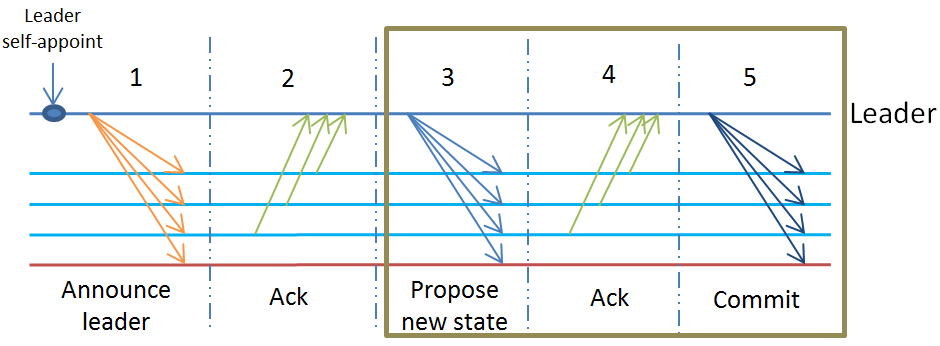
\includegraphics[width=0.8\textwidth]{images/paxos-round2}
	\end{center}
	
	Phase 2 of a very simplified Paxos round:
	\begin{itemize}
		\item The leader proposes a new value (or a state transition) (3)
		\item The leader receives the answers (4)
		\item If a majority accepts the new value, the leader orders a commit (5)
		\item Otherwise a new round must be started
	\end{itemize}
}


%%%%%%%%%%%%%%%%%%%%%%%%%%%%%%%%%%%%%%%%%%%%%%%%%%%%%%%%%%
%%%%%%%%%%%%%%%%%%%%%%%%%%%%%%%%%%%%%%%%%%%%%%%%%%%%%%%%%%
\section{Raft}

\begin{frame}
	\begin{colorblock}{blue}{lightblue}{ }
		\begin{center}
			\Huge \textbf{\texttt{Raft}}
		\end{center}
	\end{colorblock}
\end{frame}

%%%%%%%%%%%%%%%%%%%%%%%%%%%%%%%%%%%%%%%%%%%%%%%%%%%%%%%%%%
\subsection{Introduction}
\frame {\frametitle{Introduction}
	Modern implementation of a consensus protocol
	\begin{itemize}
		\item Published at Usenix 2014\cite{raft}
		\item Has been built to be easy to understand and implement
	\end{itemize}

	\vspace{7pt}

	Random facts:
	\begin{itemize}
		\item The authors released a reference C++ implementation (LogCabin)
		\item Many implementations in other languages
	\item Lots of educational material, lectures and assignments are available\footnote{These slides are based on the original Raft paper\cite{raft} and the slide deck from Michael Freedman (Princeton, COS-418).}
	\end{itemize}
}

%%%%%%%%%%%%%%%%%%%%%%%%%%%%%%%%%%%%%%%%%%%%%%%%%%%%%%%%%%
\frame {\frametitle{Introduction}
	
	\begin{itemize}
		\item Raft maintains a distributed log containing state machine commands
		\item The \emph{elected leader} handles all communication with the clients\\
		      ($\rightarrow$ no communication until a leader is elected)\\
		      and has the control on which entries are committed to the log
		\item The other nodes are passive replicators
		\item Snapshotting is used to keep the log size limited
		\item Periodic heartbeats are used to check if nodes are alive
		\item All nodes are known in advance
	\end{itemize}
}

%%%%%%%%%%%%%%%%%%%%%%%%%%%%%%%%%%%%%%%%%%%%%%%%%%%%%%%%%%
\frame {\frametitle{Node states}
	\begin{itemize}
		\item At any given time, each node is either:
		\begin{itemize}
			\item Leader: handles client requests, manages the log
			\item Follower: passively replicates the log and the state machine
			\item Candidate: transition state used during elections
		\end{itemize}
	
		\vspace{10pt}
		
		\item Normal operation, with N nodes (N must be odd):
		\begin{itemize}
			\item 1 leader
			\item N-1 follower
			\item 0 candidates
		\end{itemize}
	\end{itemize}
}

%%%%%%%%%%%%%%%%%%%%%%%%%%%%%%%%%%%%%%%%%%%%%%%%%%%%%%%%%%
\subsection{Leader election}
\frame {\frametitle{Election terms}
	\begin{center}
		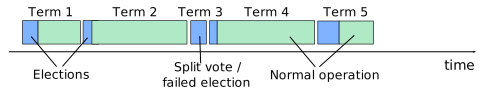
\includegraphics[width=0.8\textwidth]{images/raft-1}
	\end{center}
	\begin{itemize}
		\item Time is divided into terms, each identified by a monotonically increasing ID
		\item Each node records the term he believes to be the current one
		\item All messages are labeled with a term ID $\Rightarrow$ term IDs are used to identify obsolete information
	\end{itemize}
}

%%%%%%%%%%%%%%%%%%%%%%%%%%%%%%%%%%%%%%%%%%%%%%%%%%%%%%%%%%
\frame {\frametitle{Elections}
	How an election starts:
	\begin{itemize}
		\item Each node has a (bounded) random timer, the \emph{election timeout}
		\item If a node does not receive any leader heartbeat before the timeout, it starts the election
	\end{itemize}

	\vspace{12pt}

	The node that starts an election:
	\begin{itemize}
		\item Increments the term ID, becomes \emph{Candidate} and votes for itself
		\item Sends a request to vote to all other nodes until either:
		\begin{itemize}
			\item Receives a majority of votes $\rightarrow$ becomes \emph{Leader}
			\item Receives a message from another leader $\rightarrow$ becomes \emph{Follower}
			\item No-one wins before the election timeout expires again $\rightarrow$ starts a new election
		\end{itemize}
	\end{itemize}
}

%%%%%%%%%%%%%%%%%%%%%%%%%%%%%%%%%%%%%%%%%%%%%%%%%%%%%%%%%%
\frame {\frametitle{Election properties}
	\begin{itemize}
		\item \emph{Safety}: there is at most one winner/leader per term
		\begin{itemize}
			\item Each voter votes only once per term
			\item There cannot be two majorities in the same term
		\end{itemize}
	
		\vspace{12pt}
	
		\item \emph{Liveness}: a leader will eventually be elected
		\begin{itemize}
			\item The election is started after a random timeout
			\item The randomness guarantees there will be different candidates at different times
			\item Faults (hence new terms) happen in days/weeks/months, an election lasts milliseconds/seconds
		\end{itemize}
	\end{itemize}
}

%%%%%%%%%%%%%%%%%%%%%%%%%%%%%%%%%%%%%%%%%%%%%%%%%%%%%%%%%%
\subsection{Log replication}
\frame {\frametitle{Normal operation}
	
	\begin{center}
		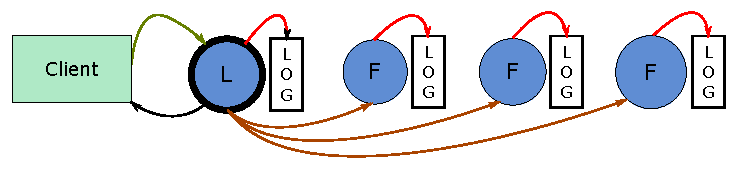
\includegraphics[width=0.8\textwidth]{images/raft-2}
	\end{center}
	
	\begin{enumerate}
		\item Clients send commands to the current leader
		\item The leader logs a new (uncommitted) entry
		\item The leader sends the new entry to all nodes in the next heartbeat
		\item Once a majority answers, the leader commits the new entry
		\item The leader answers the client
		\item The leader asks all nodes to commit the entry in the next heartbeat
		\item The nodes commit the entry in their logs
	\end{enumerate}
}

%%%%%%%%%%%%%%%%%%%%%%%%%%%%%%%%%%%%%%%%%%%%%%%%%%%%%%%%%%
\subsection{Failure scenarios}
\frame {\frametitle{What if ... the leader fails}

	Short answer:\\
	easy, after the election timeout expires a new leader is elected
	
	\vspace{10pt}
	
	What happens to uncommitted entries?
	\begin{itemize}
		\item The client will never receive the commit ack (will retry later)
		\item Uncommitted entries in the followers will eventually be overwritten by the new leader
	\end{itemize}

	\vspace{5pt}

	And when it restarts?
	\begin{itemize}
		\item It will restart as a follower
		\item It will set its internal term ID according to the first heartbeat message it receives
		\item The leader will send missing log entries
	\end{itemize}
}

%%%%%%%%%%%%%%%%%%%%%%%%%%%%%%%%%%%%%%%%%%%%%%%%%%%%%%%%%%
\frame {\frametitle{What if ... a follower fails}
	
	Short answer:\\
	nothing happens
	
	\vspace{15pt}
	
	And when it restarts?
	\begin{itemize}
		\item Same as when the leader restarts
		\item It will restart as a follower
		\item It will set its internal term ID according to the first heartbeat message it receives
		\item The leader will send missing log entries
	\end{itemize}
}

%%%%%%%%%%%%%%%%%%%%%%%%%%%%%%%%%%%%%%%%%%%%%%%%%%%%%%%%%%
\frame {\frametitle{What if ... there is a 50/50 vote}
	
	Short answer:\\
	no leader is elected, election timeout expires, new term, new election
	
	\vspace{15pt}
	
	This case is called \emph{split majority}:
	\begin{itemize}
		\item An even number of voters
		\item Two equal subsets equal in size vote for different leaders
		\item The two candidates count the votes and see that there is no majority
	\end{itemize}

	Very low probability:
	\begin{itemize}
		\item two candidates at the same time (random election timeout)
		\item messages to initiate election arrive at the same time
	\end{itemize}
}

%%%%%%%%%%%%%%%%%%%%%%%%%%%%%%%%%%%%%%%%%%%%%%%%%%%%%%%%%%
\frame {\frametitle{What if ... there is a network partition}
	
	Short answer:\\
	the majority rule ensures only half of the partition commits new entries
	
	\vspace{15pt}
	
	What happens:
	\begin{itemize}
		\item The biggest partition will elect a leader, incrementing the term ID
		\item The smaller one will be unable to do anything: all operations require a majority
	\end{itemize}
	
	And when the partition is healed?
	\begin{itemize}
		\item The minority partition will receive heartbeats with a bigger term ID
		\item The leader in the minority partition (if any), will immediately step down
		\item Uncommitted log entries will be overwritten
	\end{itemize}
}

%%%%%%%%%%%%%%%%%%%%%%%%%%%%%%%%%%%%%%%%%%%%%%%%%%%%%%%%%%
\subsection{Conclusions}
\frame {\frametitle{Learning tools and Raft summary}
	Raft interactive demos:
	\begin{enumerate}
		\item Raftscope: \url{http://bigfoot-m2.eurecom.fr/raftscope/}
		\item Secret lives of data: \url{http://thesecretlivesofdata.com/raft/}
	\end{enumerate}

	\vspace{10pt}

	\begin{itemize}
		\item Raft is a consensus protocol
		\item Consistently replicates a distributed log of state machine commands
		\item In each term a leader is elected
		\item Hard timeouts bound elections and heartbeats
		\item The leader is responsible for client communication and log replication
	\end{itemize}
}

%%%%%%%%%%%%%%%%%%%%%%%%%%%%%%%%%%%%%%%%%%%%%%%%%%%%%%%%%%
%%%%%%%%%%%%%%%%%%%%%%%%%%%%%%%%%%%%%%%%%%%%%%%%%%%%%%%%%%
\section{Implementations}
\subsection{Overview}
\frame {\frametitle{Some implementations of consensus protocols}
	\begin{itemize}
		\item ZooKeeper (ZAB)
		\vspace{4pt}
		\item Consul (Raft + Serf)
		\vspace{4pt}
		\item etcd (Raft)
		\vspace{4pt}
		\item OpenReplica/ConCoord (Paxos)
	\end{itemize}
}

%%%%%%%%%%%%%%%%%%%%%%%%%%%%%%%%%%%%%%%%%%%%%%%%%%%%%%%%%%
%%%%%%%%%%%%%%%%%%%%%%%%%%%%%%%%%%%%%%%%%%%%%%%%%%%%%%%%%%
\section{ZooKeeper}

\begin{frame}
 \begin{colorblock}{blue}{lightblue}{ }
  \begin{center}
    \Huge \textbf{\texttt{ZooKeeper}}
  \end{center}
  \end{colorblock}
\end{frame}

%%%%%%%%%%%%%%%%%%%%%%%%%%%%%%%%%%%%%%%%%%%%%%%%%%%%%%%%%%
\frame {\frametitle{Motivation}

	When building a distributed system you have two options:
	
	\begin{itemize}
		\item Build your own coordination primitive each time
		\begin{itemize}
			\item Buggy and error-prone approach
		\end{itemize}
		\item Use an external coordination system
		\begin{itemize}
			\item Adds external dependencies, more complex deployments
			\item Does not reinvent the wheel
			\item Use a well-known and tested system
		\end{itemize}
	\end{itemize}

	\vspace{10pt}

	Recent examples of coordination systems:
	\begin{itemize}
		\item Chubby from Google\cite{chubby} (lock service)
		\item Centrifuge from Microsoft\cite{Centrifuge} (Lease service)
	\end{itemize}
}

%%%%%%%%%%%%%%%%%%%%%%%%%%%%%%%%%%%%%%%%%%%%%%%%%%%%%%%%%%
\subsection{History}
\frame {\frametitle{History}
	\begin{textblock*}{50mm}(0.88\textwidth,42mm)
		
\includegraphics[width=0.3\textwidth]{images/zk-logo}
	\end{textblock*}
	
	Originally part of the Hadoop suite (2008), is now a stand-alone Apache project since 2011
	
	\vspace{10pt}
	
	Objectives\footnote{See also the Tao of ZooKeeper: \url{https://cwiki.apache.org/confluence/display/ZOOKEEPER/Tao}}:
	\begin{itemize}
		\item Provide common services needed by distributed systems
		\begin{itemize}
			\item Configuration
			\item Group management
			\item Naming
			\item Presence protocols
			\item Distributed synchronization
		\end{itemize}
		\item Have a simple interface
		\item Have a highly available architecture
	\end{itemize}
}

%%%%%%%%%%%%%%%%%%%%%%%%%%%%%%%%%%%%%%%%%%%%%%%%%%%%%%%%%%
\subsection{Architecture}
\frame {\frametitle{Architecture}
	\begin{center}
		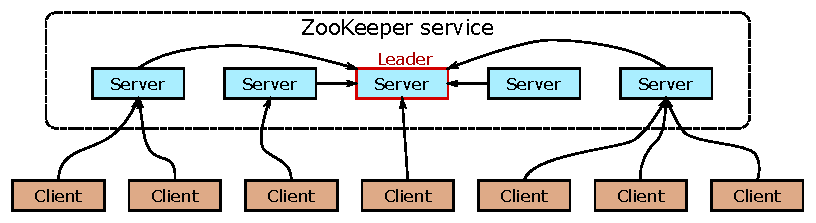
\includegraphics[width=0.9\textwidth]{images/zk-arch}	
	\end{center}

	\begin{itemize}
		\item ZooKeeper itself is distributed, for performance and fault tolerance
		\item Uses the ZAB consensus protocol
		\item Clients can talk to any server, but all update operations handled by an elected leader
		\item Data kept in-memory for performance
		\item Snapshots and transaction logs on persistent storage
	\end{itemize}
}

%%%%%%%%%%%%%%%%%%%%%%%%%%%%%%%%%%%%%%%%%%%%%%%%%%%%%%%%%%
\frame {\frametitle{Architecture - ZAB}
	The ZAB is the consensus protocol used by ZooKeeper
	\begin{itemize}
		\item It does not use state machine replication like Paxos or Raft
		\item Totally orders write requests using a majority of nodes
		\item Leader sequences the requests and invokes ZAB atomic broadcast
		\item Strictly ordered state updates are applied by non-leaders
	\end{itemize}

	\vspace{15pt}

	ZooKeeper developers focused on strong ordering guarantees for all operations\cite{Zab}
}

%%%%%%%%%%%%%%%%%%%%%%%%%%%%%%%%%%%%%%%%%%%%%%%%%%%%%%%%%%
\subsection{Data model}
\frame {\frametitle{Data model}
	\begin{center}
		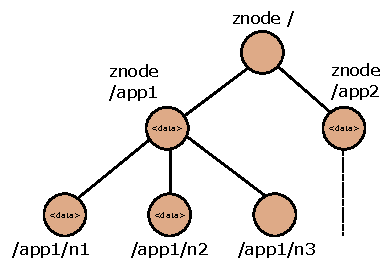
\includegraphics[width=0.6\textwidth]{images/zk-data-model}	
	\end{center}

	\begin{itemize}
		\item Hierarchical namespace (like a file system)
		\item Each data node is called \emph{znode}
		\item Any znode can contain data and have children znodes
	\end{itemize}
}

%%%%%%%%%%%%%%%%%%%%%%%%%%%%%%%%%%%%%%%%%%%%%%%%%%%%%%%%%%
\frame {\frametitle{znodes}
	Znodes can be:
	\begin{itemize}
		\item \emph{Regular}: created and destroyed by the client
		\item \emph{Ephemeral}: created by the client, but ZooKeeper will delete it if the client disconnects
		\item \emph{Sequential}: created by the client, but the name is generated by ZooKeeper using a counter
		\item \emph{Ephemeral + Sequential}: combines the two above
	\end{itemize}

	\vspace{15pt}

	Znodes have version counters that are updated each time their content changes
}

%%%%%%%%%%%%%%%%%%%%%%%%%%%%%%%%%%%%%%%%%%%%%%%%%%%%%%%%%%
\frame {\frametitle{Watches}
	A client can set a \emph{watch} on a znode. ZooKeeper will call back the client when:
	\begin{itemize}
		\item The data in the znode changes
		\item A children node is created or destroyed
	\end{itemize}

	\vspace{15pt}

	Watches are very useful to implement locks and leader elections with good performance
}

%%%%%%%%%%%%%%%%%%%%%%%%%%%%%%%%%%%%%%%%%%%%%%%%%%%%%%%%%%
\subsection{API}
\frame {\frametitle{API}
}

%%%%%%%%%%%%%%%%%%%%%%%%%%%%%%%%%%%%%%%%%%%%%%%%%%%%%%%%%%
\subsection{Conclusions}
\frame {\frametitle{Conclusions}
	\begin{itemize}
		\item ZooKeeper is a high-performance coordination service for distributed applications
		\item Internally uses the ZAB consensus protocol
		\item Clients manipulate data in form of hierarchical znodes, similar to a file system
		\item Complex, higher level primitives can be built on top of the ZooKeeper API
	\end{itemize}

	\vspace{15pt}
	
	ZooKeeper documentation: \url{https://zookeeper.apache.org/doc/r3.4.9/}
}

%%%%%%%%%%%%%%%%%%%%%%%%%%%%%%%%%%%%%%%%%%%%%%%%%%%%%%%%%%
\subsection{Laboratory session}
\frame {\frametitle{Laboratory session - leader election}
	Context:
	\begin{itemize}
		\item Sensors are streaming data to your cluster
		\item Need a central node to do aggregations, the system must be highly available
		\item Implement the leader election algorithm on top of ZooKeeper
	\end{itemize}
	
	\vspace{4pt}
	
	Objective:
	\begin{enumerate}
		\item Start three processes
		\item One of them will become the active leader
		\item Stop/crash the leader
		\item One of the surviving processes automatically takes the lead
		\item The crashed node restarts without disrupting the current leadership (bonus)
	\end{enumerate}
}

%%%%%%%%%%%%%%%%%%%%%%%%%%%%%%%%%%%%%%%%%%%%%%%%%%%%%%%%%%
%%%%%%%%%%%%%%%%%%%%%%%%%%%%%%%%%%%%%%%%%%%%%%%%%%%%%%%%%%
\begin{frame}
	\begin{colorblock}{blue}{lightblue}{ }
		\begin{center}
			\Huge \textbf{\texttt{References}}
		\end{center}
	\end{colorblock}
\end{frame}

%%%%%%%%%%%%%%%%%%%%%%%%%%%%%%%%%%%%%%%%%%%%%%%%%%%%%%%%%%
%%%%%%%%%%%%%%%%%%%%%%%%%%%%%%%%%%%%%%%%%%%%%%%%%%%%%%%%%%

\section{References}
\begin{frame}[allowframebreaks]{References}
\bibliographystyle{acm}
\bibliography{references} 
\end{frame}

\end{document}
